%%%%%%%%%%%%%%%%%%%% quantfin_detailed.tex %%%%%%%%%%%%%%%%%%%%%%%%%%%%%%%%%%%
%
% Detailed, repo-grounded research paper for QuantFin
% Format: Springer Proceedings (svproc.cls) as provided in paper/example/templates
%
%%%%%%%%%%%%%%%%%%%%%%%%%%%%%%%%%%%%%%%%%%%%%%%%%%%%%%%%%%%%%%%%%%%%%%%%%%%%%%

\documentclass{svproc}

% Template-aligned packages
\usepackage{url}
\usepackage{color}
\usepackage{makeidx}
\usepackage{graphicx}
\usepackage[misc]{ifsym}
\usepackage{multicol}
\usepackage[bottom]{footmisc}
\usepackage{tabularx}
\usepackage{multirow}
\usepackage{natbib}
\usepackage{algorithm}
\usepackage{algorithmic}
\usepackage[center]{caption}
\usepackage{longtable}
\usepackage{rotating}
\usepackage{amsmath}
\usepackage{subfigure}

\def\UrlFont{\rmfamily}

\begin{document}
\mainmatter

\title{ML-Based Decision Support System for Smart Investments}
\titlerunning{ML Decision Support for Smart Investments}

\author{Dr. Reshma Koli$^{1}$, Avanish Vadke$^{2}$, Atharva Shelke$^{3}$,\\
Abhishek Thormothe$^{4}$, Aadit Suryawanshi$^{5}$ and Prof. Harshada Sonkamble$^{6}$}
\authorrunning{Reshma Koli et al.}
\tocauthor{Reshma Koli, Avanish Vadke, Atharva Shelke, Abhishek Thormothe, Aadit Suryawanshi and Prof. Harshada Sonkamble}

\institute{\textsuperscript{123456}A.P. Shah Institute of Technology, Thane, India\\
\email{rrkoli@apsit.edu.in, avanishvadke3@apsit.edu.in, atharvashelke2@apsit.edu.in, abhishekthormothe150@apsit.edu.in, aaditsuryawanshi60@apsit.edu.in, hksonkamble@apsit.edu.in}}

\maketitle

\begin{abstract}
Retail investors and discretionary traders make decisions under uncertainty, limited information, and behavioral bias; without a measurable workflow, these decisions can lead to avoidable drawdowns. This paper presents \emph{QuantFin}, a repository-implemented, full-stack decision support system for Indian large-cap equities (Nifty~50 constituents available in the dataset). QuantFin integrates (i) robust ingestion of OHLCV time series from multi-header CSV exports; (ii) a technical-indicator feature pipeline; (iii) a multi-model prediction suite spanning regression and classification (ridge regression, logistic regression, SVM, an ARIMA baseline, and LSTM); (iv) portfolio construction via ML-driven ranking and optimization-based baselines; and (v) leakage-aware walk-forward backtesting that evaluates rebalanced strategies against a benchmark.

The emphasis of this paper is \textbf{truth-only, reproducible reporting}: all quantitative values stated are taken from saved repository artifacts and the implemented backtest engine. In the current repository state, the backend dataset contains 49 usable per-symbol CSV files spanning 1991-01-02 to 2025-10-06. For example, saved training logs for RELIANCE report test accuracy 0.5003 (logistic regression) and 0.5136 (SVM) for directional classification, and LSTM test MAPE 20.447\% for price forecasting. In a reproducible walk-forward run (monthly rebalancing, 2023-01-01 to 2024-01-01), the implemented LINEAR strategy achieved CAGR 48.31\% versus 30.60\% for the benchmark under the repository's assumptions.

\keywords{Decision Support Systems, Quantitative Finance, Walk-Forward Backtesting, Time-Series Forecasting, FastAPI, Portfolio Construction}
\end{abstract}

\section{Introduction}\label{sec:intro}
Quantitative investing systems increasingly combine statistical modeling, machine learning, and portfolio construction, but reported performance is highly sensitive to evaluation protocol. In particular, time order must be respected, and realistic constraints (e.g., rebalance cadence, capital budget) must be explicit. Recent work motivates integrating prediction with portfolio decisions while maintaining evaluation discipline \citep{aithal2023realtime, gunjan2022portfolioreview}.

QuantFin is designed as an end-to-end platform that connects these components for an Indian equity universe. Unlike isolated notebooks, QuantFin operationalizes a repeatable workflow: ingestion of OHLCV data; feature engineering; model training and inference across multiple approaches; portfolio construction and rebalancing; and walk-forward backtesting. The implementation consists of a FastAPI backend (data + ML + portfolio services) and a React/TypeScript dashboard.

\textbf{Contributions.} This work contributes:
\begin{itemize}
\item A repository-implemented architecture for interactive quantitative analysis (FastAPI backend + React/Vite frontend).
\item A leakage-aware walk-forward backtest engine that enforces date cutoffs at each rebalance date.
\item A multi-model baseline suite (linear/logistic/SVM/LSTM and an ARIMA baseline in the codebase) and multiple portfolio baselines (ML ranking, model-weighted, mean--variance, risk parity).
\item A reproducibility-first reporting approach in which claimed results are anchored to saved JSON artifacts and generated figures in the repository.
\end{itemize}

\textbf{Scope and non-claims.} QuantFin is a prototype research system. The repository includes a validation report indicating the system is not production-ready at the time of writing; therefore, this paper avoids operational claims (e.g., deployment reliability) and focuses on implemented methodology and reproducible outputs.

\section{Related Work}\label{sec:rw}
QuantFin builds on themes from (i) end-to-end ML decision support, (ii) stock ranking and recommendation, (iii) classical vs deep time-series baselines, and (iv) portfolio optimization.

\textbf{End-to-end portfolio decision support.} Aithal \emph{et al.}\ \citep{aithal2023realtime} describe integrating prediction with portfolio management. QuantFin adopts this framing but emphasizes explicit walk-forward evaluation.

\textbf{Stock ranking and recommendation.} Ranking-based selection is a practical decision interface for portfolios \citep{saha2021stockranking}. QuantFin similarly converts predictions into per-asset scores and selects top-$K$ candidates at each rebalance date.

\textbf{Classical vs deep baselines.} Comparative baselines including ARIMA and deep sequence models are common in financial forecasting \citep{gao2021arimadeep, karlis2021lstmfusion}. QuantFin exposes both families within one pipeline.

\textbf{Optimization baselines.} Reviews emphasize the role of covariance estimation and constraints in mean--variance and related methods \citep{gunjan2022portfolioreview}. QuantFin includes optimization-based baselines, while explicitly documenting simplifying assumptions where they exist in the repository.

\textbf{Rebalancing and learning-based policies.} Reinforcement learning approaches motivate periodic rebalancing and sequential decision framing \citep{lim2022dynamicrebalancing, ma2023tcr}. QuantFin does not implement RL, but adopts a rebalance-schedule evaluation protocol.

\section{System Overview}\label{sec:system}
QuantFin is a full-stack system with three layers:
\begin{itemize}
\item \textbf{Data + preprocessing layer:} loads per-symbol OHLCV CSV files and normalizes heterogeneous headers.
\item \textbf{Model + decision layer:} computes technical indicators, trains multiple model families, and converts predictions into allocations using ranking and optimization baselines.
\item \textbf{Serving + UI layer:} exposes FastAPI endpoints consumed by a React/TypeScript dashboard for interactive analysis and backtesting.
\end{itemize}

\subsection{Backend services and APIs}\label{sec:api}
The backend is organized around services that power REST endpoints. The repository exposes functional surfaces for (i) analytics and training summaries, (ii) prediction and portfolio recommendation, (iii) walk-forward backtesting, and (iv) portfolio reporting. The paper focuses on the behavior of these services as implemented, rather than presenting a hypothetical API.

\subsection{API surface (selected endpoints)}\label{sec:api_surface}
Table~\ref{tab:api_surface} lists representative endpoints drawn from the repository routers. This is not intended to be exhaustive; rather, it documents the implemented interface that supports training, inference, portfolio operations, and backtesting.

\begin{table}[h!]
\centering
\caption{Selected API endpoints (from implemented routers).}
\label{tab:api_surface}
\begin{tabularx}{\textwidth}{|l|l|X|}
\hline
Router & Prefix & Examples \\
\hline
Analytics & \texttt{/api/analytics} & \texttt{POST /models/train}, \texttt{GET /models/training-status}, \texttt{GET /candlestick/\{symbol\}}, \texttt{GET /kpis} \\
Portfolio & \texttt{/api/portfolio} & \texttt{GET /summary}, \texttt{GET /performance}, \texttt{POST /rebalance}, \texttt{GET /strategy-comparison} \\
Predictions & \texttt{/api/predictions} & \texttt{GET /symbols}, \texttt{POST /predict}, \texttt{POST /portfolio}, \texttt{GET /model/\{symbol\}/\{model\_type\}} \\
Backtest & \texttt{/api/backtest} & \texttt{POST /run}, \texttt{GET /health} \\
\hline
\end{tabularx}
\end{table}

\subsection{Artifacts and reproducibility}\label{sec:artifacts}
QuantFin is accompanied by machine-readable artifacts (JSON summaries, cached results) that enable reproducible reporting. This paper references:
\begin{itemize}
\item Dataset summary describing symbol coverage and date ranges.
\item Saved training summaries containing per-model metrics.
\item Backtest summaries containing risk/return metrics and series outputs.
\item Figures generated by repository scripts (equity curve and drawdown).
\end{itemize}

\section{Data and Preprocessing}\label{sec:data}
QuantFin operates on daily OHLCV time series stored as CSV files (one file per symbol). In the current repository state, there are 49 usable per-symbol CSV files. The global date range across these files is 1991-01-02 to 2025-10-06 (as reported by the repository's dataset summary artifact).

\subsection{Multi-header CSV normalization}\label{sec:multiheader}
Market data exports frequently include metadata rows or multi-row headers. QuantFin addresses this by skipping non-data rows and coercing values into a canonical schema with columns \texttt{Date, Open, High, Low, Close, Volume}. The normalized result is sorted by date and cached to reduce repeated I/O.

\begin{algorithm}[h!]
\caption{Multi-header OHLCV normalization (repo-aligned)}
\label{alg:normalize}
\begin{algorithmic}[1]
\REQUIRE Raw CSV file $f$ for a symbol
\ENSURE Clean dataframe with \texttt{Date, Open, High, Low, Close, Volume}
\STATE Read $f$ while skipping a fixed number of header rows (export-dependent)
\STATE Parse the first column as \texttt{Date}; drop rows with invalid dates
\STATE Coerce numeric columns (Open/High/Low/Close/Volume); drop invalid rows
\STATE Sort by \texttt{Date} ascending and de-duplicate as needed
\STATE Return normalized dataframe
\end{algorithmic}
\end{algorithm}

\subsection{Dataset summary}\label{sec:dataset_summary}
Table~\ref{tab:dataset} summarizes the dataset scope as captured in repository artifacts.

\begin{table}[h!]
\centering
\caption{Dataset scope (from repository dataset summary artifact).}
\label{tab:dataset}
\begin{tabular}{|l|l|}
\hline
Number of usable symbols & 49 \\
Global start date & 1991-01-02 \\
Global end date & 2025-10-06 \\
Data type & Daily OHLCV per symbol \\
\hline
\end{tabular}
\end{table}

\section{Feature Engineering}\label{sec:features}
QuantFin implements a technical-indicator pipeline that produces both return-based features and common indicators used in technical analysis. Given close price $P_t$, simple and log returns are defined as:
\begin{equation}
r_t = \frac{P_t - P_{t-1}}{P_{t-1}},\quad \ell_t = \log\left(\frac{P_t}{P_{t-1}}\right).
\end{equation}

Features include moving averages (SMA/EMA), MACD, RSI, Bollinger bands, rolling volatility, momentum, lagged returns, and volume-derived features. The goal is to provide a consistent feature matrix for classical models and a sequence representation for LSTM.

\section{Model Suite}\label{sec:models}
QuantFin includes multiple baselines to support comparison and ablation.

\subsection{Ridge regression (price/return regression)}
Ridge regression is used as a regularized linear baseline for regression targets. Regularization controls overfitting on correlated technical indicators.

\subsection{Logistic regression (direction classification)}
Logistic regression is used as a baseline classifier for up/down movement. Besides accuracy, saved artifacts include precision, recall, F1, and AUC.

\subsection{Support vector machines (SVM)}
An RBF-kernel SVM baseline is used for direction classification with hyperparameter selection recorded in artifacts.

\subsection{ARIMA baseline (classical time-series)}
The repository codebase includes an ARIMA baseline to provide a classical univariate comparator. Where metrics are not present in saved training summaries, this paper does not report ARIMA numbers.

\subsection{LSTM (sequence forecasting)}
An LSTM model is used for sequence forecasting with a fixed sequence length and a limited number of epochs in the stored run. Saved artifacts include regression metrics (MSE/RMSE/MAE/R\,$^2$) and MAPE.

\subsection{Repo-grounded training example (RELIANCE)}\label{sec:reliance}
To illustrate the repository's stored outputs, Table~\ref{tab:reliance_metrics} summarizes metrics for RELIANCE taken directly from the saved training summary artifact.

\begin{table}[h!]
\centering
\caption{Saved training metrics for RELIANCE (from repository artifacts).}
\label{tab:reliance_metrics}
\begin{tabular}{|l|l|l|}
\hline
Model & Task & Test metric(s) \\
\hline
Ridge (linear\_reg) & Regression & MAE $\approx$ 0.0742; $R^2 \approx -0.335$ \\
LogReg & Classification & Accuracy $\approx$ 0.5003; AUC $\approx$ 0.5073 \\
SVM (RBF) & Classification & Accuracy $\approx$ 0.5136; AUC $\approx$ 0.5051 \\
LSTM & Forecasting & MAPE $\approx$ 20.447\% \\
\hline
\end{tabular}
\end{table}

\subsection{Additional stored regression baselines across symbols}\label{sec:more_training}
In addition to the per-model training summary for RELIANCE, the repository contains a separate training-results artifact capturing linear regression baselines for multiple symbols under a fixed train/test split date. Table~\ref{tab:linear_multi} reports the stored values for three symbols (RELIANCE, TCS, INFY), including sample counts and test-set regression metrics.

\begin{table}[h!]
\centering
\caption{Stored linear regression results across symbols (split date 2023-01-01; from repository artifact).}
\label{tab:linear_multi}
\begin{tabular}{|l|r|r|r|r|}
\hline
Symbol & Train samples & Test samples & Test MAE & Test $R^2$ \\
\hline
RELIANCE & 6768 & 662 & 0.04936 & -0.13660 \\
TCS & 4778 & 662 & 0.04899 & -0.13379 \\
INFY & 6771 & 662 & 0.05707 & -0.01326 \\
\hline
\end{tabular}
\end{table}

\section{Decision Layer: Portfolio Construction}\label{sec:portfolio}
QuantFin converts model outputs into portfolio decisions using (i) ranking-based selection and (ii) optimization-based baselines.

\subsection{Ranking-based selection and allocation}\label{sec:ranking}
At each rebalance date, the system computes a per-asset score derived from predicted return and a confidence signal. Assets are filtered to remove non-positive expected returns, and the top-$K$ are selected; weights are assigned equally among selected assets. This design keeps the decision rule transparent and makes backtest comparisons interpretable.

\subsection{Optimization baselines}\label{sec:opt}
QuantFin includes mean--variance and risk-parity style baselines. Where applicable, the repository uses covariance estimated from historical returns in the backtest engine. Separately, the online prediction service includes a simplified constant-correlation covariance construction; this distinction is important for accurate interpretation.

\section{Walk-Forward Backtesting}\label{sec:backtest}
The backtest engine evaluates strategies in a leakage-aware walk-forward manner. The key principle is that each rebalance decision is made using information available up to that date; realized returns over the subsequent interval update portfolio value.

\begin{algorithm}[h!]
\caption{Leakage-aware walk-forward backtest (high-level)}
\label{alg:backtest}
\begin{algorithmic}[1]
\REQUIRE Start/end dates, rebalance schedule, capital $V_0$, strategy $\pi$
\STATE Initialize portfolio value $V \leftarrow V_0$
\FOR{each rebalance date $d_t$ in the schedule}
  \STATE Build features from data up to $d_t$ (no look-ahead)
  \STATE Obtain model predictions and compute allocation weights $w_t = \pi(\text{features}, \text{predictions})$
  \STATE Apply realized returns over $(d_t, d_{t+1}]$ to update $V$
\ENDFOR
\STATE Compute summary metrics (CAGR, Sharpe, drawdown) and return time series
\end{algorithmic}
\end{algorithm}

\subsection{Example reproducible run (2023-01 to 2024-01)}\label{sec:run}
The repository includes artifacts for a monthly-rebalanced walk-forward run from 2023-01-01 to 2024-01-01 with capital 100,000 and top-$N=10$ selection. Table~\ref{tab:backtest_summary} reports the stored summary metrics.

\begin{table}[h!]
\centering
\caption{Backtest summary (monthly rebalancing, 2023-01-01 to 2024-01-01; stored artifact).}
\label{tab:backtest_summary}
\begin{tabular}{|l|r|r|}
\hline
Metric & LINEAR strategy & Benchmark \\
\hline
CAGR (\%) & 48.31 & 30.60 \\
Sharpe & 3.043 & 1.752 \\
Sortino & 14.244 & 5.038 \\
Max drawdown (\%) & -1.165 & -4.181 \\
Final value & 148271.84 & 130578.43 \\
\hline
\end{tabular}
\end{table}

\subsection{Backtest variants (stored summaries)}\label{sec:variants}
To probe sensitivity to rebalance cadence and evaluation window, the repository includes a variants summary artifact for the LINEAR strategy across multiple configurations. Table~\ref{tab:variants} reports these stored summaries. (Note: some risk metrics may appear as 0 or N/A for short horizons or small numbers of rebalance periods, reflecting the artifact values.)

\begin{table}[h!]
\centering
\caption{Stored backtest variants for LINEAR strategy (from repository variants summary artifact).}
\label{tab:variants}
\begin{tabular}{|p{4.0cm}|r|r|r|r|r|}
\hline
Variant & CAGR (\%) & Sharpe & Volatility & Max DD (\%) & Rebalances \\
\hline
Monthly (2023-01 to 2024-01) & 48.31 & 3.043 & 11.71 & -1.17 & 12 \\
Quarterly (2023-01 to 2024-01) & 40.54 & 3.725 & 27.97 & 0.00 & 4 \\
Monthly (2022-01 to 2024-01) & 37.47 & 1.796 & 15.80 & -5.31 & 24 \\
\hline
\end{tabular}
\end{table}

\subsection{Visualization}\label{sec:viz}
Figures~\ref{fig:equity} and \ref{fig:drawdown} show the stored equity curve and drawdown plots for the same run.

\begin{figure}[h!]
\begin{center}
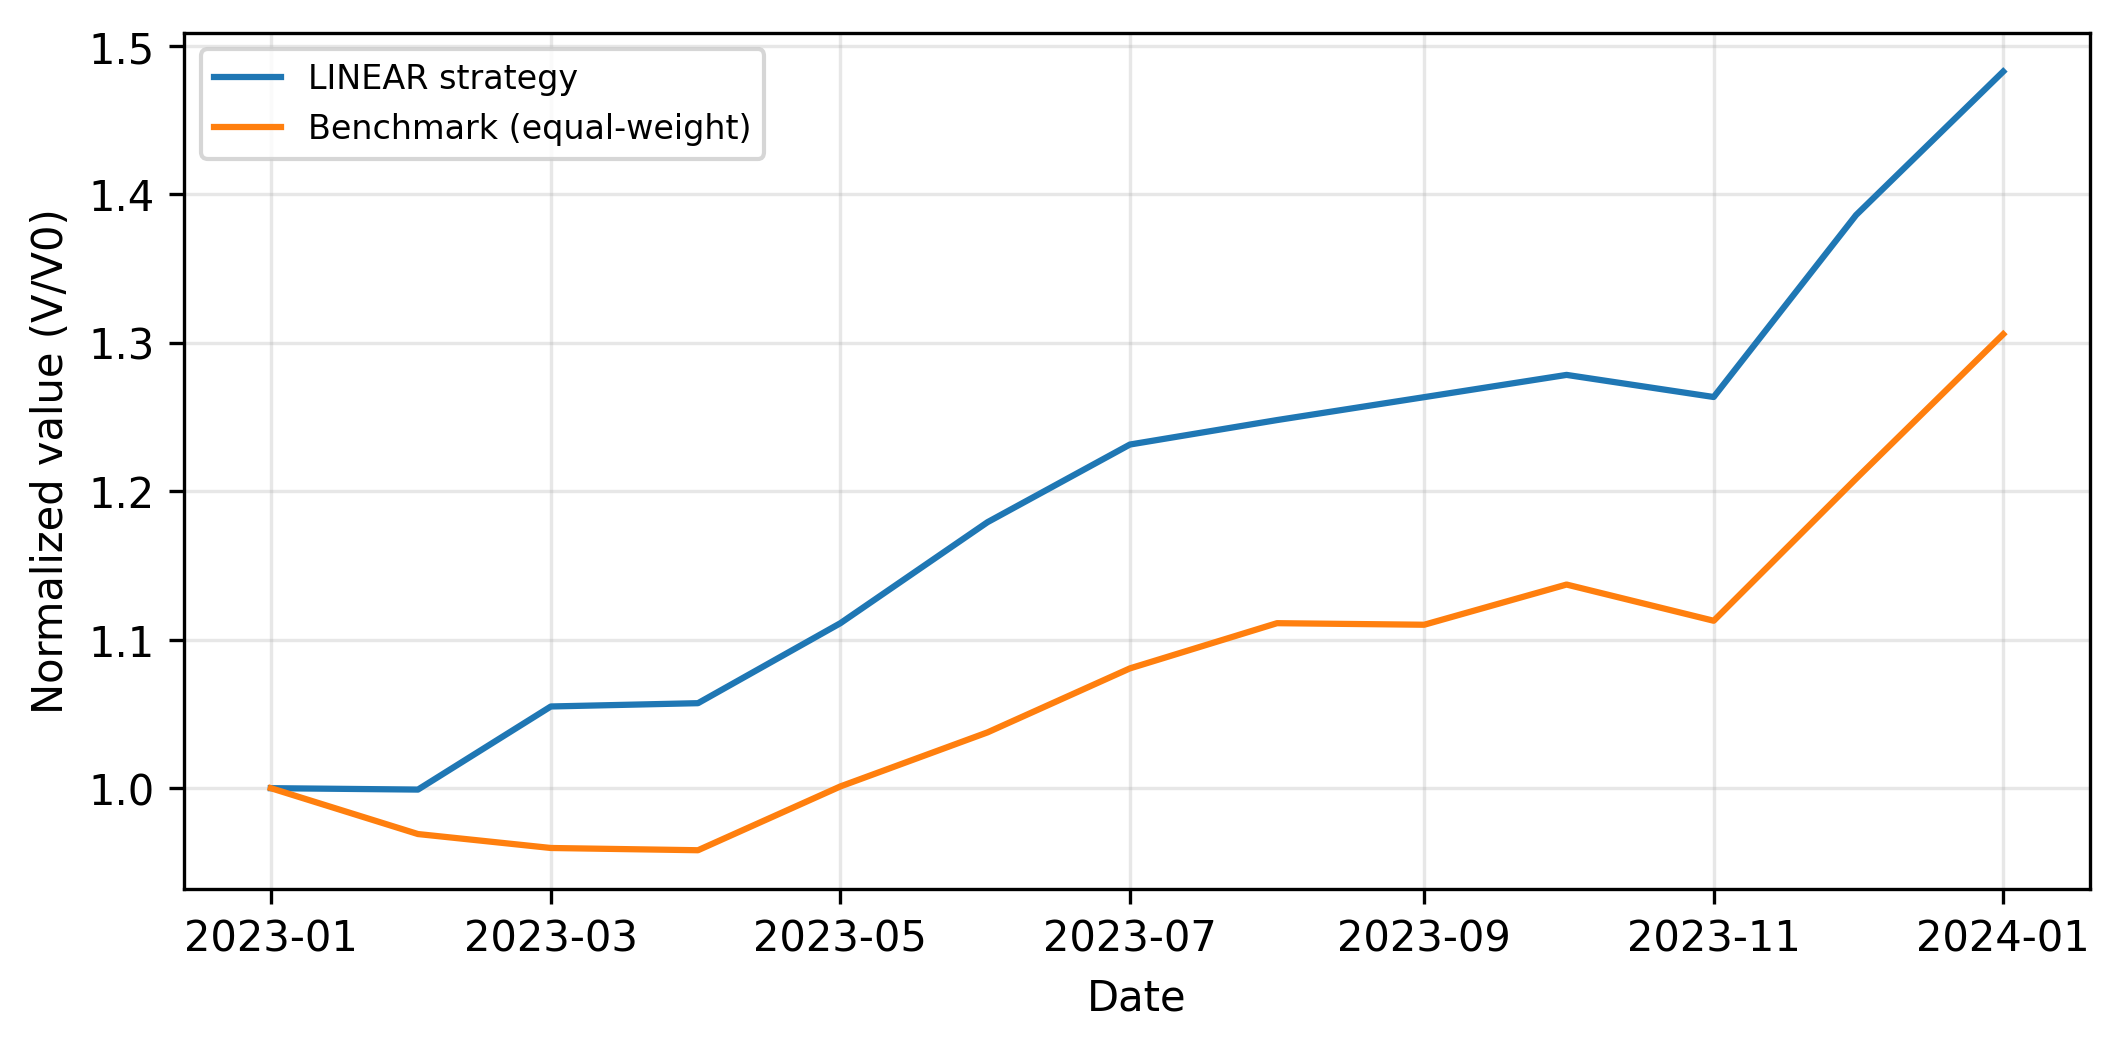
\includegraphics[width=0.9\textwidth]{figures/equity_curve_2023_2024_linear.png}
\caption{Equity curve: LINEAR strategy vs benchmark (stored figure).}
\label{fig:equity}
\end{center}
\end{figure}

\begin{figure}[h!]
\begin{center}
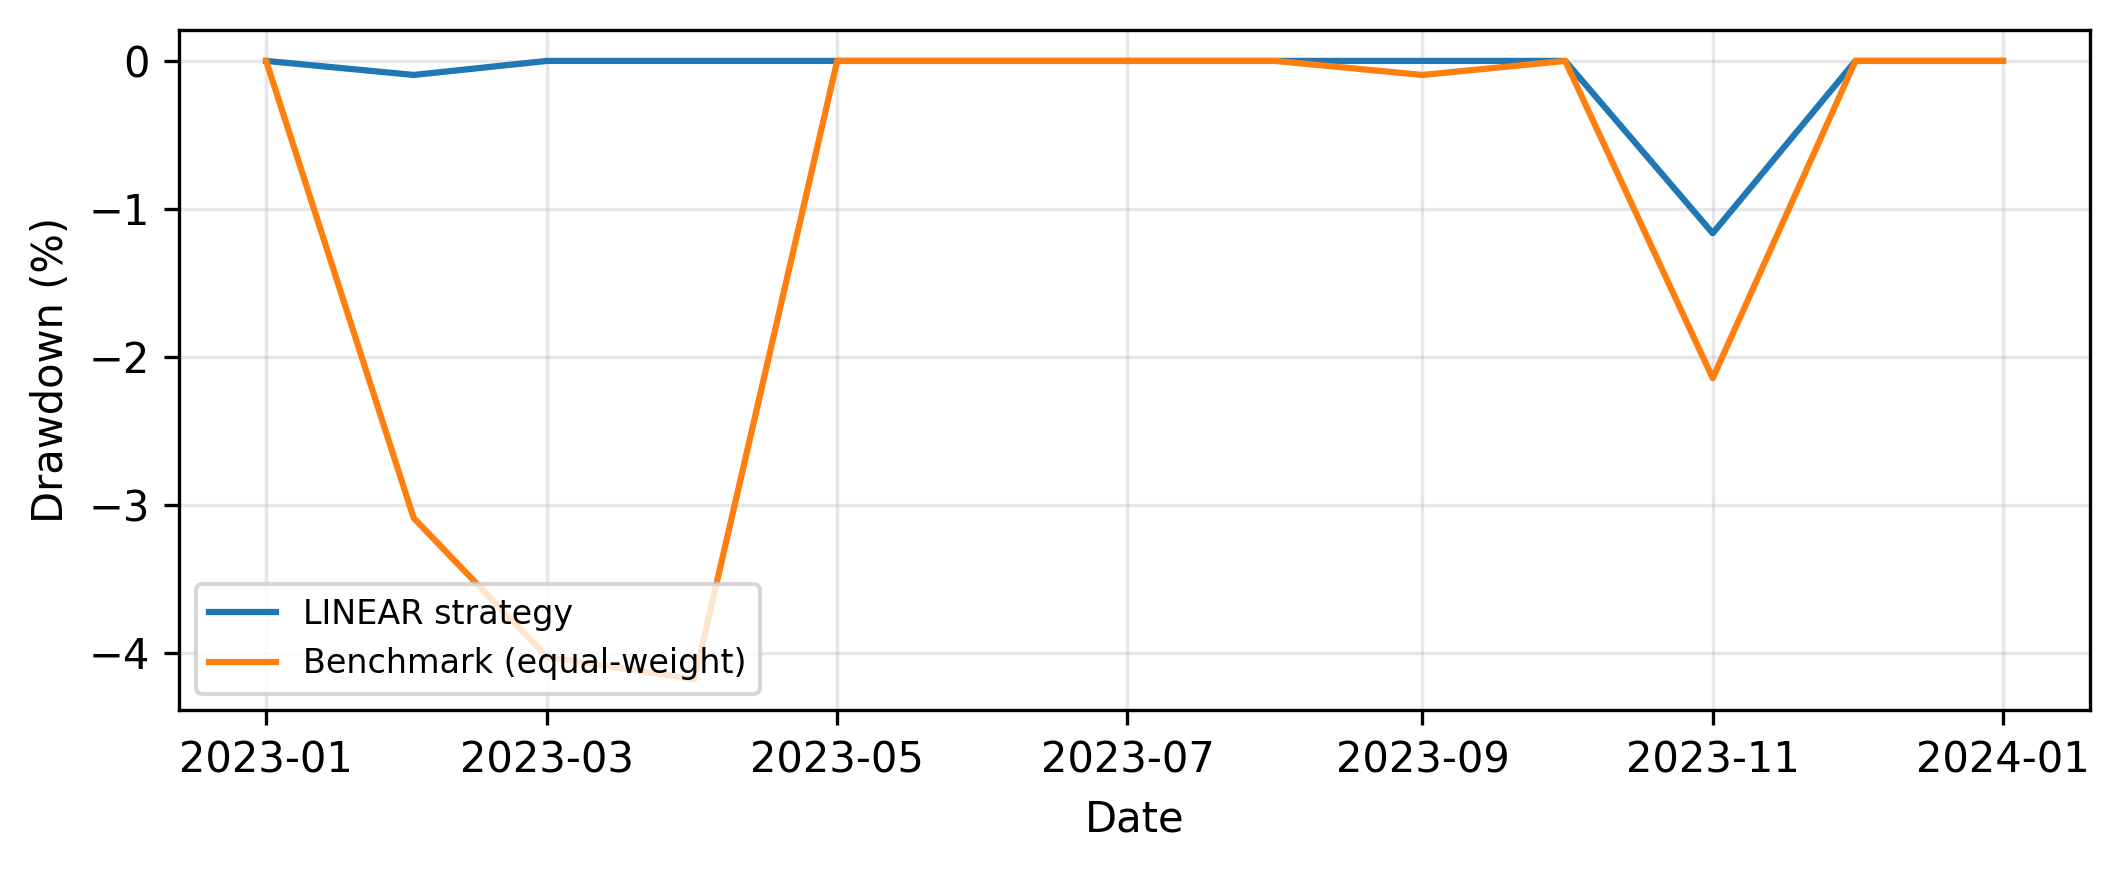
\includegraphics[width=0.9\textwidth]{figures/drawdown_2023_2024_linear.png}
\caption{Drawdown: LINEAR strategy vs benchmark (stored figure).}
\label{fig:drawdown}
\end{center}
\end{figure}

\section{Frontend and User Interaction}\label{sec:frontend}
QuantFin includes a React/TypeScript dashboard that calls backend endpoints to visualize prices, model outputs, allocations, and backtest results. The frontend is designed to provide:
\begin{itemize}
\item interactive selection of symbols and model families,
\item inspection of training summaries and metrics,
\item portfolio composition and health views,
\item execution and visualization of walk-forward backtests.
\end{itemize}
The paper does not claim user-study outcomes; instead, it documents the implemented interaction surface.

\section{Engineering Validation Snapshot}\label{sec:validation}
Because QuantFin is a research prototype, it is important to explicitly document engineering status rather than imply production readiness. The repository includes a validation report artifact that executes a small suite of environment and integration checks. Table~\ref{tab:validation} summarizes the stored outcomes, and the report marks \texttt{production\_ready} as \texttt{false}.

\begin{table}[h!]
\centering
\caption{Validation report snapshot (from repository validation artifact).}
\label{tab:validation}
\begin{tabular}{|l|c|p{8.0cm}|}
\hline
Check & Passed & Details (stored) \\
\hline
Environment Setup & Yes & Packages installed; 49 data files found \\
API Route Registration & No & attempted relative import beyond top-level package \\
Backtester Module & No & 0 passed, 0 failed (suite did not run successfully) \\
Integration Tests & No & Backtester.\_\_init\_\_() missing required argument: \texttt{models\_dir} \\
\hline
\end{tabular}
\end{table}

\section{Limitations and Threats to Validity}\label{sec:limits}
This work is constrained by the repository's scope and artifacts.
\begin{itemize}
\item \textbf{Transaction costs and slippage:} the stored backtest assumptions do not include explicit transaction costs or market impact; therefore returns may be optimistic relative to real trading.
\item \textbf{Model comparability:} models solve different tasks (regression, classification, forecasting). Direct comparison requires careful alignment of targets and metrics.
\item \textbf{Covariance estimation details:} some optimization paths use simplified covariance assumptions (notably in the online prediction service), while the backtest engine can estimate covariance from historical returns. Results should be interpreted with this distinction.
\item \textbf{Engineering readiness:} repository validation artifacts indicate the system is not production-ready; operational robustness is outside this paper's claims.
\end{itemize}

\section{Conclusion and Future Work}\label{sec:con}
This paper presented QuantFin, a full-stack, repository-implemented decision support system for equity investing that combines multi-header data ingestion, technical-indicator features, multiple ML baselines, and leakage-aware walk-forward backtesting. By grounding claims in saved artifacts, the paper provides a reproducible description of both methodology and observed outcomes.

Future work includes (i) richer multi-asset feature representations (e.g., explicit cross-asset structure), (ii) cost-aware backtesting with realistic frictions, (iii) better calibrated uncertainty estimates for ranking and allocation, and (iv) expanding stored evaluation artifacts to cover all implemented baselines (including ARIMA) across a broader symbol set.

\bibliographystyle{plain}
\bibliography{review}
\end{document}
